%
% CHAPTER 3.- Codes and Information
%

\chapterimage{Morse_key.pdf}

\chapter{Coding}
\label{chap:Coding}

\begin{quote}
\begin{flushright}
\emph{Information is the resolution of uncertainty.}\\
Claude Shannon
\end{flushright}
\end{quote}
\bigskip

In this section we are going to review the conceptual ideas and main results behind coding theory and the related area of information theory.

Coding is the process of describing a sequence of symbols from some alphabet by a sequence of symbols from another alphabet. Coding has many practical applications, such as error detection, cryptography, or telecommunications. Here our interest is in data compression, that is, encoding a message using fewer symbols than its original representation, without losing any information. Compression algorithms reduce the size of messages by identifying unnecessary elements and removing it, usually by means of computing and eliminating statistical redundancy. For example, data compression can be achieved by assigning shorter descriptions to the most frequent symbols from the source, and longer descriptions to the less frequent symbols. A particular type of codes, the prefix-free codes, will play a central role in this book. Prefix-free codes allow us to link coding theory with probability theory, a link that will be very useful in the context of the theory of nescience.

Information theory proposes that the amount of information we get when some event happens is the logarithm of the inverse of the probability of that event. In this sense, the theory assumes that information is equivalent to surprise: the more unlikely is an event, the more information we get when the event occurs. We are not going to use that interpretation of information in our theory of nescience, but we will extensively use another concept from information theory: entropy. Entropy quantifies the amount of uncertainty involved in the value of a random variable or the outcome of a random process. Entropy is important to us because it establishes a limit to the compression of texts: it is not possible to find a code with average word length smaller that the entropy of the source alphabet.

There exists many interesting concepts derived from entropy, like join entropy, conditional entropy, or mutual information. However, these concepts are more relevant in the context of communication, because they allow us to solve the problem of how to transmit information in a reliable manner over a noisy channel. Here, they are introduced for completeness purposes, and to compare them with our own definitions of join nescience and conditional nescience.

%
% Section: Codes and their properties
%

\section{Coding}
\label{Codes}

Intuitively, coding refers to the process of losslessly describing a sequence of symbols (a message) coming from some alphabet by other sequences of symbols coming from a (potentially) different alphabet. There is no general agreement about what it is exactly a code, since different authors propose different definitions. Fortunately, the definition of prefix-free code, the kind of codes required by the theory of nescience, is a standard one.

Let $\mathcal{S}=\left\{ s_{1},s_{2},\ldots,s_{q}\right\}$ be a finite set called \emph{source alphabet}, and $\mathcal{X}=\left\{ x_{1}, x_{2}, \ldots, x_{r} \right\}$ a finite set called \emph{code alphabet}.

\begin{definition}[Code]
A \emph{code} for $\mathcal{S}$ is a total function $C:\mathcal{S}\rightarrow\mathcal{X}^{+}$. If $(s,x) \in C$ we say that $s$ is the \emph{source symbol} and $x$ is the \emph{code word}. If $C$ is an injective function we say that the code is \emph{nonsingular}.
\end{definition}

Nonsingularity allows us to unambiguously describe the individual symbols of the source alphabet. For the rest of this book, whenever we talk about a code we mean a nonsingular code. Moreover, without any loss of generality, we will restrict ourselves to \emph{binary codes}, that is, $\mathcal{X} = \mathcal{B}$.

The property of nonsingularity can also be applied to strings of symbols. In order to do that, we have to extend the concept of code from symbols to strings.

\begin{definition}
The \emph{extension of order $n$} of a code $C$ is a function $C^{n}:\mathcal{S}^{n}\rightarrow\mathcal{B}^{+}$ defined as $C^{n}(s_{i_1} \ldots s_{i_n}) = C(s_{i_1}) \ldots C(s_{i_n})$, where $C(s_{i_1}) \ldots C(s_{i_n})$ is the concatenation of the code words corresponding to the symbols of the string $s_{i_1} \ldots s_{i_n} \in {S}^{n}$. An extension of order $n$ of a code $C$ is \emph{nonsingular} if the function $C^{n}$ is injective.
\end{definition}

If it is clear from the context, we will also use the word \emph{code} to refer to a nonsingular extension of order $n$ of a code, and the elements of $S^{n}$ will be called \emph{source words}.

\begin{example}
\label{ex:nonsingularity}
The code $C(a)=0$, $C(b)=00$, $C(c)=01$ and $C(d)=11$ is a nonsingular code, but its extension of order 2 is singular, since, for example, $C(ab)=C(ba)=000$.
\end{example}

As we have seen in Example \ref{ex:nonsingularity} not all nonsingular codes have nonsigular extensions, that is, it might happen that we are not able to decode the original messages given their encoded versions. Unique decodability is a highly desirable property of codes.

\begin{definition}
A code $C$ is called \emph{uniquely decodable} if its order $n$ extension $C^{n}$ is nonsingular for all $n$.
\end{definition}

Next proposition provides an alternative characterization of the unique decodability of codes.

\begin{proposition}
A code $C$ is uniquely decodable if, and only if, the function $C^{+}:\mathcal{S}^{+}\rightarrow\mathcal{B}^{+}$ is injective.
\end{proposition}
\begin{proof}
If the function $C^{+}$ is injective, the restriction to $C^{n}$ must be injective for all $n$. Now let assume that $C^{n}$ is nonsingular for all $n$ and let's prove that $C^{+}$ must be nonsingular by contradiction: select two source words $s_{1} \in \mathcal{S}_n$ and $s_{2} \in \mathcal{S}_m$, $n \neq m$, and assume that they have the same code word $C^{+}(s_{1}) = C^{+}(s_{2})$, then construct the symbols $s_{3} = s_{1}s_{2}$ and $s_{4} = s_{2}s_{1}$, both $s_{3}$ and $s_{4}$ have the same length and $C^{+}(s_{3}) = C^{+}(s_{4})$ which is a contradiction with the fact that $C^{n+m}$ must be singular.
\end{proof}

\begin{example}
\label{ex:uniquely-decodable}
The code $C(a)=0$, $C(b)=01$, $C(c)=011$ and $C(d)=0111$ is a uniquely decodable code. For example, the code word $0010011$ uniquely corresponds to the source word $abac$. The unique decodability is achieved because the $0$ symbol, that plays the role of a comma, separating code words.
\end{example}

Next definition introduces the concept of prefix-free codes. Prefix-free codes will play a critical role in the computation of the amount of algorithmic information of an arbitrary string (described in Chapter \ref{chap:Algorithmic_Information}), and in our own theory of nescience. Prefix-free codes also allow us to link coding theory and probability theory through the Kraft inequality (Theorem \ref{th:Kraft-Inequality}). Note that we prefer the name \emph{prefix-free code} to the more standard name of \emph{prefix code}, since the former fits more accurately to the concept it names.

\begin{definition}[Prefix-free Code]
\label{def:Prefix-free-Code}
A code $C$ is \emph{prefix-free} if $C(s_{i})$ is not a prefix of $C(s_{j})$ for all $i,j\left(1\leq i,j\leq q\right)$.
\end{definition}

\begin{example}
\label{ex:prefix-free}
The code $C(a)=0$, $C(b)=10$, $C(c)=110$ and $C(d)=1110$ is a prefix-free code. The $0$ symbol also plays the role of a comma as it was the case of Example \ref{ex:uniquely-decodable}, but its new position at the end of the code words guarantees is what makes the code prefix-free.
\end{example}

Fortunately, prefix-free codes are also uniquely decodable, as next proposition proves.

\begin{proposition}
Let $C$ be a prefix-free code, then $C$ is uniquely decodable.
\end{proposition}
\begin{proof}
Let $C$ be a fixed length code, $C^n$ its extension of order $n$, and $r = r_1 r_2 \ldots r_n$ and $s = s_1 s_2 \ldots s_n$ two source words such that $r \ne s$ but $C^n(r) = C^n(s)$. Then, we have that $C(r_1) \ldots C(r_n) = C(s_1) \ldots C(s_n)$, or equivalently that $r_1^1 \ldots r_1^{i_1} \ldots r_n^1 \ldots r_1^{i_n} = s_1^1 \ldots s_1^{j_1} \ldots s_n^1 \ldots s_1^{j_n}$. If $i_1 \leq j_1$ we have that $r_1$ is a prefix of $c_1$, and if $i_1 > j_1$ the $s_1$ is a prefix of $r_1$, whihc is a contradiction with the fact that $C$ is prefix-free.
\end{proof}

From an engineering point of view it is highly convenient to have codes whose source symbols can be decoded as soon as the corresponding code words are received, that is, it is not necessary to wait for the next code word in order to decode the current symbol. For example, given the code described in Example \ref{ex:uniquely-decodable}, after receiving the sequence $011$ the source symbol could be a $c$ or a $d$. Prefix-free codes present this property, this is why some authors prefer to call them \emph{instantaneous codes}.

Figure \ref{fig:Classification-Codes} provides a graphical representation of the relation about the different types of codes that have been introduced in this section.

\begin{figure}[h]
\centering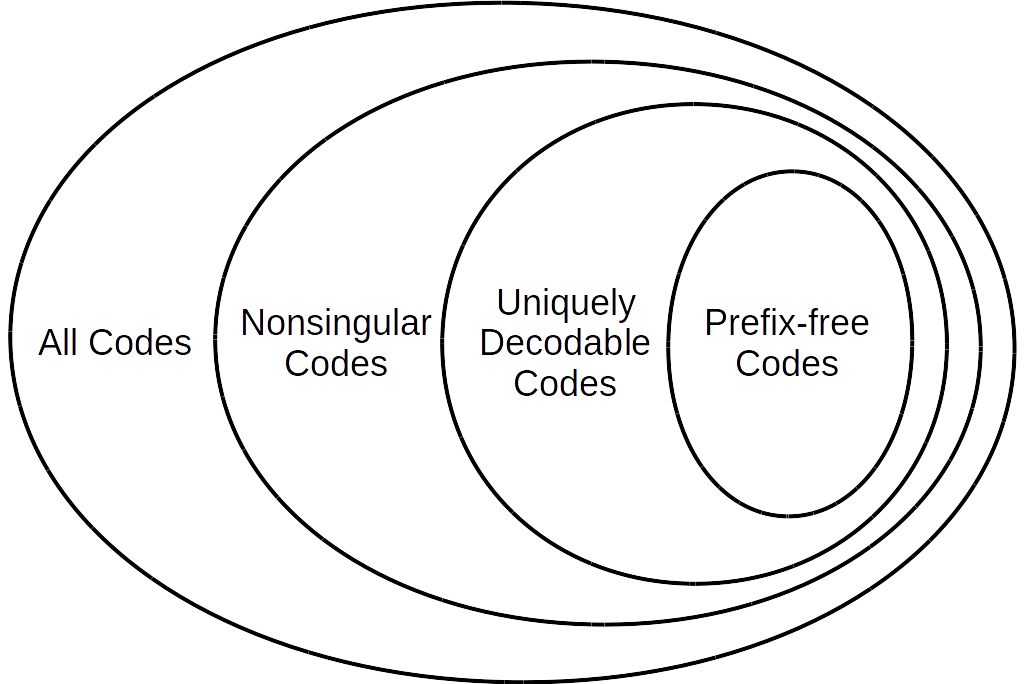
\includegraphics[scale=0.3]{Codes}
\caption{\label{fig:Classification-Codes}Classification of Codes}
\end{figure}

Another interesting type of codes are fixed length codes. We will use fixed length codes to compute the length of a text when we assume that there is any regularity we can use to compress the text.

\begin{definition}
\label{def:Fixed-Length-Codes}
If all the code words of a code have the same length we say that the code is a \emph{fixed length code}.
\end{definition}

Fixed codes have the property of being prefix-free.

\begin{proposition}
Let $C$ be a fixed-length code, then $C$ is prefix-free.
\end{proposition}
\begin{proof}
Let $C$ be a fixed length code, and $C(s_i)$ and $C(s_j)$ the code words of two arbitrary source words $s_i$ and $s_j$. Assume that $C(s_i) <_p C(s_j)$, given the fact that $l(C(s_i)) = l(C(s_j))$ we have that $C(s_i) = C(s_j)$ and so, the code $C$ is prefix-free.
\end{proof}

Of course, the converse of the previous proposition does not hold.

%
% Section: Kraft Inequality
%

\section{Kraft Inequality}

The Kraft inequality provides a sufficient, and necessary, condition for the existence of a prefix-free code given a set of code words lengths. Among other things, Kraft inequality is important because if we take an exponential of the length of each codeword, the resulting set of values look like a probability mass function, that is, they sum less than or equal to one.

\begin{theorem}[Kraft Inequality]
\label{th:Kraft-Inequality}
Let $\mathcal{L}=\left\{ l_{1},l_{2},\ldots,l_{q}\right\}$ a set of lengths, $l_{i}\in\mathbb{N}$, then there exists a binary prefix-free code $C$ whose code words have the lengths of $\mathcal{L}$ if, and only if,
\[
\sum_{l_{i}\in\mathcal{L}}2^{-l_{i}}\leq1
\]
\end{theorem}
\begin{proof}

Consider a binary tree whose branches are labeled with the symbols of the code alphabet, in such a way that the path from the root to the leaves traces out the symbols of a codeword. The prefix-free condition implies that nodes containing codewords cannot have descendants. An example of such a tree, for the code described in Example \ref{ex:prefix-free}, is shown in Figure \ref{fig:Prefix-Free-Tree}. 

\begin{figure}[h]
\centering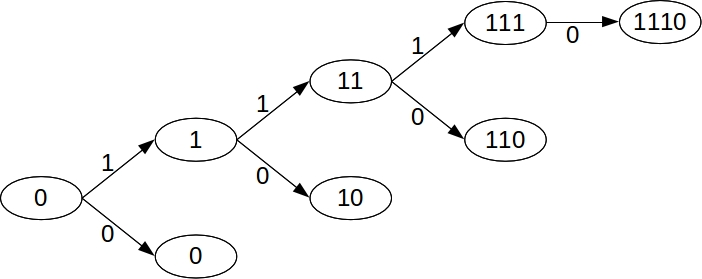
\includegraphics[scale=0.4]{PrefixFreeTree2}
\caption{\label{fig:Prefix-Free-Tree}Prefix-free Tree}
\end{figure}

Let $l_{max}=\max \left\{ l_{1},l_{2},\ldots,l_{q}\right\}$, that is, the length of the longest codeword from the set of lengths. There will be at most $2^{l_{max}}$ leaf nodes in the tree, but at level $l_{i}$ we have to prune $2^{l_{max} - l_{i}}$ leafs, since the code is prefix-free. Summing over all the codewords lengths, we have that the total number of pruned leafs must be less or equal that the maximum number of leafs, that is
\[
\sum_{l_{i}\in\mathcal{L}}2^{l_{max}-l_{i}} \leq 2^{l_{max}}
\]
or, equivalently
\[
\sum_{l_{i}\in\mathcal{L}}2^{-l_{i}} \leq 1
\]
which is exactly the inequality we are trying to prove.

Conversely, given any set of codewords lengths $\mathcal{L}=\left\{ l_{1},l_{2},\ldots,l_{q}\right\}$ that satisfy the Kraft inequality, we can always construct a binary tree, like the one in the Figure \ref{fig:Prefix-Free-Tree}. Label the first node (lexicographcally) of depth $l_{1}$ as code word 1, and remove its descendants from the tree. Then label the first remaining node of depth $l_{2}$ as codeword 2, and so on. Proceeding this way, we construct a prefix code with the specified lengths.

\end{proof}

Given a code $C$ whose code words lengths $\mathcal{L}$ satisfy the Kraft inequality does necessarily means that the code is prefix-free, since what the inequality states is that there exist a prefix-free code with those word lengths, not that all codes with those word lengths are prefix-free.

\begin{example}
\label{ex:not-prefix-fix}
The code $C(a)=0$, $C(b)=111$, $C(c)=110$ and $C(d)=100$ satisfies the Kraft inequality, but it is not prefix-free.
\end{example}

Kraft's inequality allows us to compare how efficient are the different codes available for the same source alphabet.

\begin{definition}
Let $C_1:\mathcal{S}\rightarrow\mathcal{X}^{+}$ and $C_2:\mathcal{S}\rightarrow\mathcal{X}^{+}$ two different codes. We say that code $C_1$ is \emph{more efficient} than code $C_2$ if for all $s \in \mathcal{S}$ we have that $l(C_1(s)) \leq l(C_2(s))$, and there exist at least one $s' \in \mathcal{S}$ such that $l(C_1(s')) < l(C_2(s'))$.
\end{definition}

\begin{example}
The code described in Example \ref{ex:not-prefix-fix} is more efficient than the code of Example \ref{ex:prefix-free}. Of course, the problem with the code described in Example \ref{ex:not-prefix-fix} is that it is not prefix-free, but since it satisfy the Kraft's inequality, we know that there must exists another code with the same code word lengths that it is prefix free. For example, $C(a)=0$, $C(b)=10$, $C(c)=110$ and $C(d)=111$.
\end{example}

We are interested in the most efficient possible codes.

\begin{definition}
A code $C$ is \emph{complete} if there does not exists a code $C'$ that is more efficient that $C$.
\end{definition}

It turns out that the Kraft's inequality provides a very useful characterization of complete codes.

\begin{proposition}
A code $C$ is complete if, and only if, its code word lengths $\mathcal{L}=\left\{ l_{1},l_{2},\ldots,l_{q}\right\}$ satisfy the property:
\[
\sum_{l_{i}\in\mathcal{L}}2^{-l_{i}} = 1
\]
\end{proposition}
\begin{proof}
{\color{red} TODO: To be done}
\end{proof}

As we said above, in the theory of nescience we are mostly interested in prefix-fix codes. That might appear as a limitation, since it sounds more reasonable to use the more general class of uniquely decodable codes. However, such limitation does not exists, since, as next theorem proves, uniquely decodable codes also satisfy Kraft's inequality. That is, for any uniquely decodable code there exists a prefix-free code with exactly the same code word lengths. In the theory of nescience we are not interested in the codes themselves, but in code lengths.

\begin{theorem}[McMillan Inequality]
\label{th:Kraft-Inequality}
Let $\mathcal{L}=\left\{ l_{1},l_{2},\ldots,l_{q}\right\}$ a set of lengths, $l_{i}\in\mathbb{N}$, then there exists a uniquely decodable code $C$ whose code words have the lengths of $\mathcal{L}$ if, and only if,
\[
\sum_{l_{i}\in\mathcal{L}}2^{-l_{i}} \leq 1
\]
\end{theorem}
\begin{proof}
{\color{red} TODO: To be done}
\end{proof}

%
% Section: Entropy
%

\section{Entropy}
\label{sec:Entropy}

In this section we are going to introduce the concept of \emph{entropy}, as a measure of the uncertainty of a random variable. Entropy is a very difficult to grasp concept that can be applied in many different contexts, such as communications, statistics, finance, etc. Here we are interested in entropy because it will allow us to identify codes with the shortest possible average length.

Let $A = \{a_1, a_2, \ldots, a_n\}$ a finite set, and $X$ a random variable defined over the set $A$ with probability mass function $p(a)$.

\begin{definition}[Entropy]
The \emph{entropy} of the random variable $X$, denoted by $H(X)$ and measured in \emph{bits}, is defined as:
\[
H(X) = \sum_{a \in A} p(a) \log \frac{1}{p(a)}
\]
\end{definition}

Note that the entropy of $X$ does not depend on the individual elements of $A$, but on their probabilities. It is easy to show that $H(X) \geq 0$ since $0 \leq p(a) \leq 1$ implies that $-\log p(a) \geq 0$. In case of $p(a_i) = 0$ for some $i$, the value of the corresponding summand $0 \log 0$ is taken to be $0$, which is consistent with the limit $\lim_{p\to 0^+} p \log p = 0$. If we change the base of the logarithm to $u$, entropy will be scaled by a factor of $\log_u 2$ (see Equation \ref{eq:change_base_logarithm}).

\begin{example}
Let $X$ a random variable defined over the set $A = \{a_1, a_2\}$, with values $p(a_1) = q$ and $p(a_2) = 1-q$. Then, the entropy of $X$ is given by:
\[
H(X) = q \log \frac{1}{q} + (1-q) \log \frac{1}{1-q}
\]
Figure \ref{fig:entropy_function} shows the entropy of $X$ for different values of $q$. If $q=0$ or $q=1$ the entropy is 0, that is, there is no uncertainty about which value of $A$ we will get. The maximum value of $H$ is 1, and it is reached when $q=1/2$; that is, we could say that 1 bit is the uncertainty associated to two equally probable symbols.
\end{example}

\begin{figure}[h]
\centering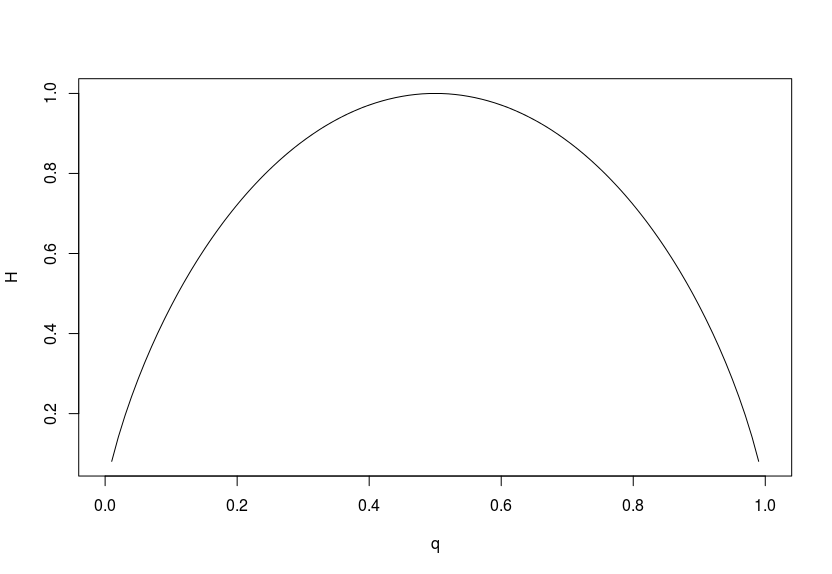
\includegraphics[scale=0.4]{entropy_function}
\caption{\label{fig:entropy_function}Binary Entropy Function}
\end{figure}

Next proposition shows that the maximum value for entropy is the logarithm of the number of symbols of $A$, and that this value is reached when all the symbols have the same probability.

\begin{proposition}
\label{prop:maximum_entropy}
Given the random variable $X$ we have that $H(X) \leq \log n$, and $H(X) = \log n$ if, and only if, $p(a_1) = p(a_2) = \ldots = p(a_n)$.
\end{proposition}
\begin{proof}
Consider the expression:
\[
\log n - H(X) = \sum_{i=1}^n p(a_i) \log n - \sum_{i=1}^n p(a_i) log {\frac{1}{p(a_i)}} = \sum_{i=1}^n p(a_i) \log n p(a_i)
\]
Applying property \ref{eq:change_base_logarithm} we have that:
\[
\log n - H(X) = \log e \sum_{i=1}^n p(a_i) \ln n p(a_i)
\]
And applying property \ref{eq:natural_logarithm_inequality} (equalling $x = 1 / n p(a_i)$):
\[
\log n - H(X) \geq \log e \sum_{i=1}^n p(a_i) \left( 1 - \frac{1}{n p(a_i)} \right) \geq \log e \left( \sum_{i=1}^n p(a_i) - \frac{1}{n} \sum_{i=1}^n \frac{p(a_i)}{p(a_i)} \right) \geq 0
\]
Which proves that $H(X) \leq \log n$.

The inequality becomes an equality if, and only if, $p(a_i) = 1 / n$ (given that the inequality \ref{eq:natural_logarithm_inequality} becomes an equality if, and only if, $x=1$).

\end{proof}

\begin{example}
If we choose a random symbol from $A$ according to the probability mass function $p$, entropy would be the minimum expected number of binary questions (Yes/No questions) required to identify the selected symbol. If the symbols of $A$ are equiprobable, the expected number of questions is maximal and equal to $\log d(A)$.
\end{example}

We can extend the concept of entropy to a pair of random variables by means of using the joint probability mass function. In this way, the joint entropy will be a measure of the uncertainty associated to both variables. Let $A = \{a_1, a_2, \ldots, a_n\}$ and $B = \{b_1, b_2, \dots, b_m\}$ two finite sets, and $X$ and $Y$ two random variables defined over the sets $A$ and $B$ respectively, with probability mass function $p(a)$ and $p(b)$, and joint probability mass function $p(a, b)$.

\begin{definition}
The \emph{joint entropy} of the random variables $A$ and $B$, denoted by $H(A, B)$, is defined as:
\[
H(A, B) = \sum_{a \in A} \sum_{b \in B} p(a, b) \log \frac{1}{p(a, b)}
\]
\end{definition}

Since $p(a, b) = p(b, a)$ we have that the joint entropy does not depend of the order in which the random variables are selected, that is $H(A, B) = H(B, A)$. We can provide a similar definition for the joint entropy of a set of $n$ random variables $A_1, A_2, \ldots, A_n$ using the joint probability mass function $p(a_1, a_2, \ldots, a_n)$.

Adding a second random variable whose outcome is not know might increase the entropy, as following proposition proves.

\begin{proposition}
We have that
\[
H(A, B) \geq \max \left( H(A), H(B) \right)
\]
\end{proposition}
\begin{proof}
\[
H(A, B) = \sum_{a \in A} \sum_{b \in B} p(a,b) \log \frac{1}{p(a,b)} \geq \sum_{a \in A} \sum_{b \in B} p(a,b) \log \frac{1}{p(a)} = \sum_{a \in A} p(a) \log \frac{1}{p(a)} = H(A)
\]
In the same way we can prove that $H(A, B) \geq H(B)$. Combining both inequalities we get the desired result.
\end{proof}

The joint entropy of two random variables cannot be greater that the sum of their individual entropies.

\begin{proposition}
\label{prop:joint_entropy}
We have that $H(A, B) \leq H(A) + H(B)$ and $H(A, B) = H(A) + H(B)$ if, and only if, $p(a)$ and $p(b)$ are statistically independent.
\end{proposition}
\begin{proof}
{\color{red} TODO: Prove without using the concept of conditional entropy nor mutual information.}
\end{proof}

% Conditional Entropy

The next derived concept from entropy that we are going to introduce is conditional entropy. Conditional entropy measures the uncertainty of a random variable given that the value of another random variable is known.

\begin{definition}
The \emph{conditional entropy} of the random variable $B$ given the random variable $A$, denoted by $H(B \mid A)$, is defined as:
\[
H(B \mid A) = \sum_{a \in A} \sum_{b \in B} p(a, b) \log \frac{1}{p(b \mid a)}
\]
\end{definition}

Since $p(b \mid a) \neq p(a \mid b)$ we have that $H(B \mid A) \neq H(A \mid B)$. If $H(B \mid A) = 0$ we have that the value of $B$ is completely determined by the value of $A$.

Next proposition proves that knowing the value of a second random variable can never increase the uncertainty of a random variable.

\begin{proposition}
Given the random variables $X$ and $Y$, we have that $H(Y \mid X) \leq H(Y)$, and $H(Y \mid X) = H(Y)$ if, and only if, $p(a)$ and $p(b)$ are independent.
\end{proposition}
\begin{proof}
\begin{multline}
H(Y \mid X) = \sum_{a \in A} \sum_{y \in B} p(a, b) \log \frac{1}{p(b \mid a)} = \sum_{a \in A} \sum_{b \in B} p(a, b) \log \frac{p(a)}{p(a, b)} \\
\notag = \sum_{a \in A} \sum_{b \in B} p(a, b) \log p(a) - \sum_{a \in A} \sum_{b \in B} p(a, b) \log p(a, b) = -H(X) + H(X, Y)
\end{multline}
Applying Propositon \ref{prop:joint_entropy} we have that $H(Y \mid X) = H(X, Y) - H(X) \leq H(X) + H(Y) - H(X) = H(Y)$.
The iff equality is also proved by applying Proposition \ref{prop:joint_entropy}.
\end{proof}

From an intuitive point of view we could expect that the uncertainty associated to a pair of random variables must be equal to the uncertainty of one of them plus the uncertainty of the second given that we know the outcome of the first one.

\begin{proposition}[Chain rule]
\label{prop:chain_rule_entropy}
Given the random variables $X$ and $Y$ we have that $H(X, Y) = H(X) + H(Y \mid X)$.
\end{proposition}
\begin{proof}
\begin{multline}
H(Y, X) = \sum_{a \in A} \sum_{b \in B} p(a, b) \log \frac{1}{p(a, b)} = \sum_{a \in A} \sum_{b \in B} p(a, b) \log \frac{1}{p(a) p(a \mid b)} \\
\notag = \sum_{a \in A} \sum_{b \in B} p(a, b) \log \frac{1}{p(a)} + \sum_{a \in A} \sum_{b \in B} p(a, b) \log \frac{1}{p(a \mid b)} = H(X) + H(Y \mid X)
\end{multline}
\end{proof}

% Mutual information

The last derived concept of entropy we are going to see is mutual information. Intuitively, the mutual information of two random variables $X$ and $Y$ measures the information that $X$ and $Y$ share, that is, how much knowing one of these variables reduces the uncertainty about the other.

\begin{definition}
The \emph{mutual information} of the random variable $X$ and $Y$, denoted by $I(X ; Y)$, is defined as:
\[
I(X ; Y) = \sum_{a \in A} \sum_{b \in B} p(a, b) \log \frac{p(a, b)}{p(a) p(b)}
\]
\end{definition}

Since $p(a, b) = p(b, a)$ we have that $I(X ; Y) = I(Y ; X)$, that is, the order of the random variables does not affect the concept of mutual information.

Next proposition shows that mutual information is a positive quantity, and it is equal to 0 if, and only if, the random variables are independent.

\begin{proposition}
Given the random variables $X$ and $Y$ we have that $I(X ; Y) \geq 0$, and $I(X ; Y) = 0$ if, and only if, the variables $X$ and $Y$ are independent.
\end{proposition}
\begin{proof}
{\color{red} TODO: to be done}
\end{proof}

{\color{red} Introduce this proposition}

\begin{proposition}
Given the random variables $X$ and $Y$, we have that:
\[
I(X;Y) = H(X) - H(X \mid Y) = H(Y) - H(Y \mid X)
\]
\end{proposition}
\begin{proof}
{\color{red} TODO: to be done}
\end{proof}

{\color{red} Introduce this proposition}

\begin{proposition}
Given the random variables $X$ and $Y$, we have that:
\[
I(X;Y) = H(X) + H(Y) - H(X, Y)
\]
\end{proposition}
\begin{proof}
{\color{red} TODO: to be done}
\end{proof}

{\color{red} Prove that $I(\mathcal{S}; \mathcal{S}) = H(\mathcal{S})$}

{\color{red} Use the Venn diagrams in this example}

\begin{example}
\end{example}

%
% Section: Optimal Codes
%

\section{Optimal Codes}
\label{sec:Optimal-Codes}

{\color{red} TODO: Explain the concept of unversal code. Give an example.}

Lets fix $\mathcal{S}=\left\{ s_{1},s_{2},\ldots,s_{q}\right\}$ a finite source alphabet, and $P$ a probability distribution defined over the elements of $S$.

\begin{definition}
The \emph{expected length} for a code $C$, denoted by $L_{C}$, is defined as
\[
L_{C} = \sum_{i=1}^{q} P(s_{i})l_{i}
\]
where $\mathcal{L} = \left\{ l_{1},l_{2},\ldots,l_{q}\right\}$ are the lengths of the code words of $C$. If $C$ is clear from the context, we will denote $L_{C}$ by $L$.
\end{definition}

We are interested in finding a code $C$ that minimizes the expected length $L$ of the code words $\mathcal{L}$ given the probability distribution $P$. This code $C$ will allow us to compress the messages written with $S$, that is, to reduce the number of symbols required to write the messages.

\begin{definition}
The redundancy of a code is defined as
\[
\eta = \frac{H(\mathcal(S)}{L}
\]
\end{definition}

Of course, our goal is to minimize the redundancy of codes. Next definition provides a formal definition of this concept:

\begin{definition}
A code $C$ is \emph{compact} if its average length $L$ is less than or equal to the average length of all the other codes for the same source alphabet and code alphabet.
\end{definition}

{\color{red} TODO: explain the relation between comple and copact codes}

Next theorem states that the entropy of the probability distibution $P$ poses a limit to the average length of prefix-free codes.

\begin{theorem}
\label{th:optimal_codes}
The expected length $L_{C}$ of any prefix-free $r$-ary code, given the probability distribution $P$, is greater than or equal to the entropy of $P$, that is
\[
H_{r}(P) \leq L_{C}
\]
with equality if, and only if, $r^{-l_{i}} = P_{i}$ for all $0 \leq i \leq q$.
\end{theorem}
\begin{proof}
\end{proof}

\begin{definition}
A probability distribution is called \emph{D-adic} if each of the probabilities is equal to $D^n$ for some $n$.
\end{definition}

\begin{corollary}
We have the equality in the theorem if, and only if, the distribution of X is D-adic.
\end{corollary}
\begin{proof}
{\color{red} TODO}
\end{proof}

{\color{red} TODO: Explain how this relates to complete codes}

{\color{red} TODO: Mention that optimal codes are random}

{\color{red} Mention that in practice we will non-integer codeword lengths. Show that, on average, the length of the encoded string will be less than 1 bit than usind a code with codewords with integer lengths} 

%
% Section: Huffman Algorithm
%

\section{Huffman Algorithm}
\label{sec:Huffman-Algorithm}

{\color{red} This section should be about compression algorithms. Not sure if only about algorithms based on information theory, or generic compression algorithms. Depends of what we need in practice}

{\color{red} Mention that Huffman is not necessarily the optimal compression algorithm}

From a practical point of view, there exists an algorithm, called \emph{Huffman algorithm}, that provides a method to build compact prefix-free codes given a probability distribution. For simplicity, we will study first the particular case of constructing binary prefix-free codes, and later I will provide its generalization to the case of D-ary prefix-free codes.

\begin{algorithm}
\caption{Huffman Algorithm}
\label{alg:Huffman}
\begin{algorithmic}
\Procedure{Huffman}{$Q$}
    \State $T \gets$ empty tree
    \For {$i \gets 1, d(Q) - 1$}
        \State allocate a new node $z$
        \State z.left = x = EXTRACT-MIN(Q)
        \State z.rigth = y = EXTRACT-MIN(Q)
        \State z.freq = x.freq + y.freq
        \State INSERT(Q, z)
    \EndFor
    \State \textbf{return} $T$
\EndProcedure
\end{algorithmic}
\end{algorithm}

The algorithm (see Algorithm \ref{alg:Huffman}) expects as input a source alphabet $\mathcal{S}=\left\{ s_{1},s_{2},\ldots,s_{q}\right\}$ and their corresponding probabilities $P = \left\{ p_{1}, p_{2}, \ldots, p_{q} \right\}$. For simplicity, we will merge both sets into a single one $Q = \left\{ (s_{1}, p_{1}), (s_{2}, p_{2}), \ldots, (s_{q}, p_{q}) \right\}$. The algorithm works by constructing a binary tree $T$, similar to the one used in the proof of Theorem \ref{th:Kraft-Inequality}. The algorithm requires $d(Q) - 1$ iterations to finish. During each iteration, the two elements with the lowest probability are selected and removed from set $Q$, and a new tree node $z$ is created, with the addition of the removed values, and added to the set $Q$. Once the tree has been constructed, we have to perform a tree transversal assigning a $0$ to each left branch, and a $1$ to each right branch, until we reach a leaf.

\begin{example}
Assume we have the source alphabet $\mathcal{S}=\left\{a, b, c, d, e, f\right\}$ with the associated probabilities $P = \left\{0.35, 0.16, 0.08, 0.12, 0.06, 0.23 \right\}$. In Figure \label{fig:Huffman-Algorithm} are depicted the contents of the set $Q$ and the tree $T$ for each iteration of the algorithm. At the end of the algorithm, if we perform a traversal of the $T$ tree, we will get the following prefix-free compact code for the source alphabet $S$: 

\bigskip

\centering
\begin{tabular}{l l}
\toprule
\textbf{Source Word} & \textbf{Code Word} \\
\midrule
a & 11   \\
b & 00   \\
c & 1011 \\
d & 100  \\
e & 1010 \\
f & 01   \\
\bottomrule
\end{tabular}

\bigskip

The expected length of the code is $L = 2.4$ , and its entropy is $\mathcal{H} \approx 2.34$. Since the set of probabilities is not D-adic ...

% Q: Shall I mention the expected length of a uniform code?

\end{example}

\begin{figure}[h]
\centering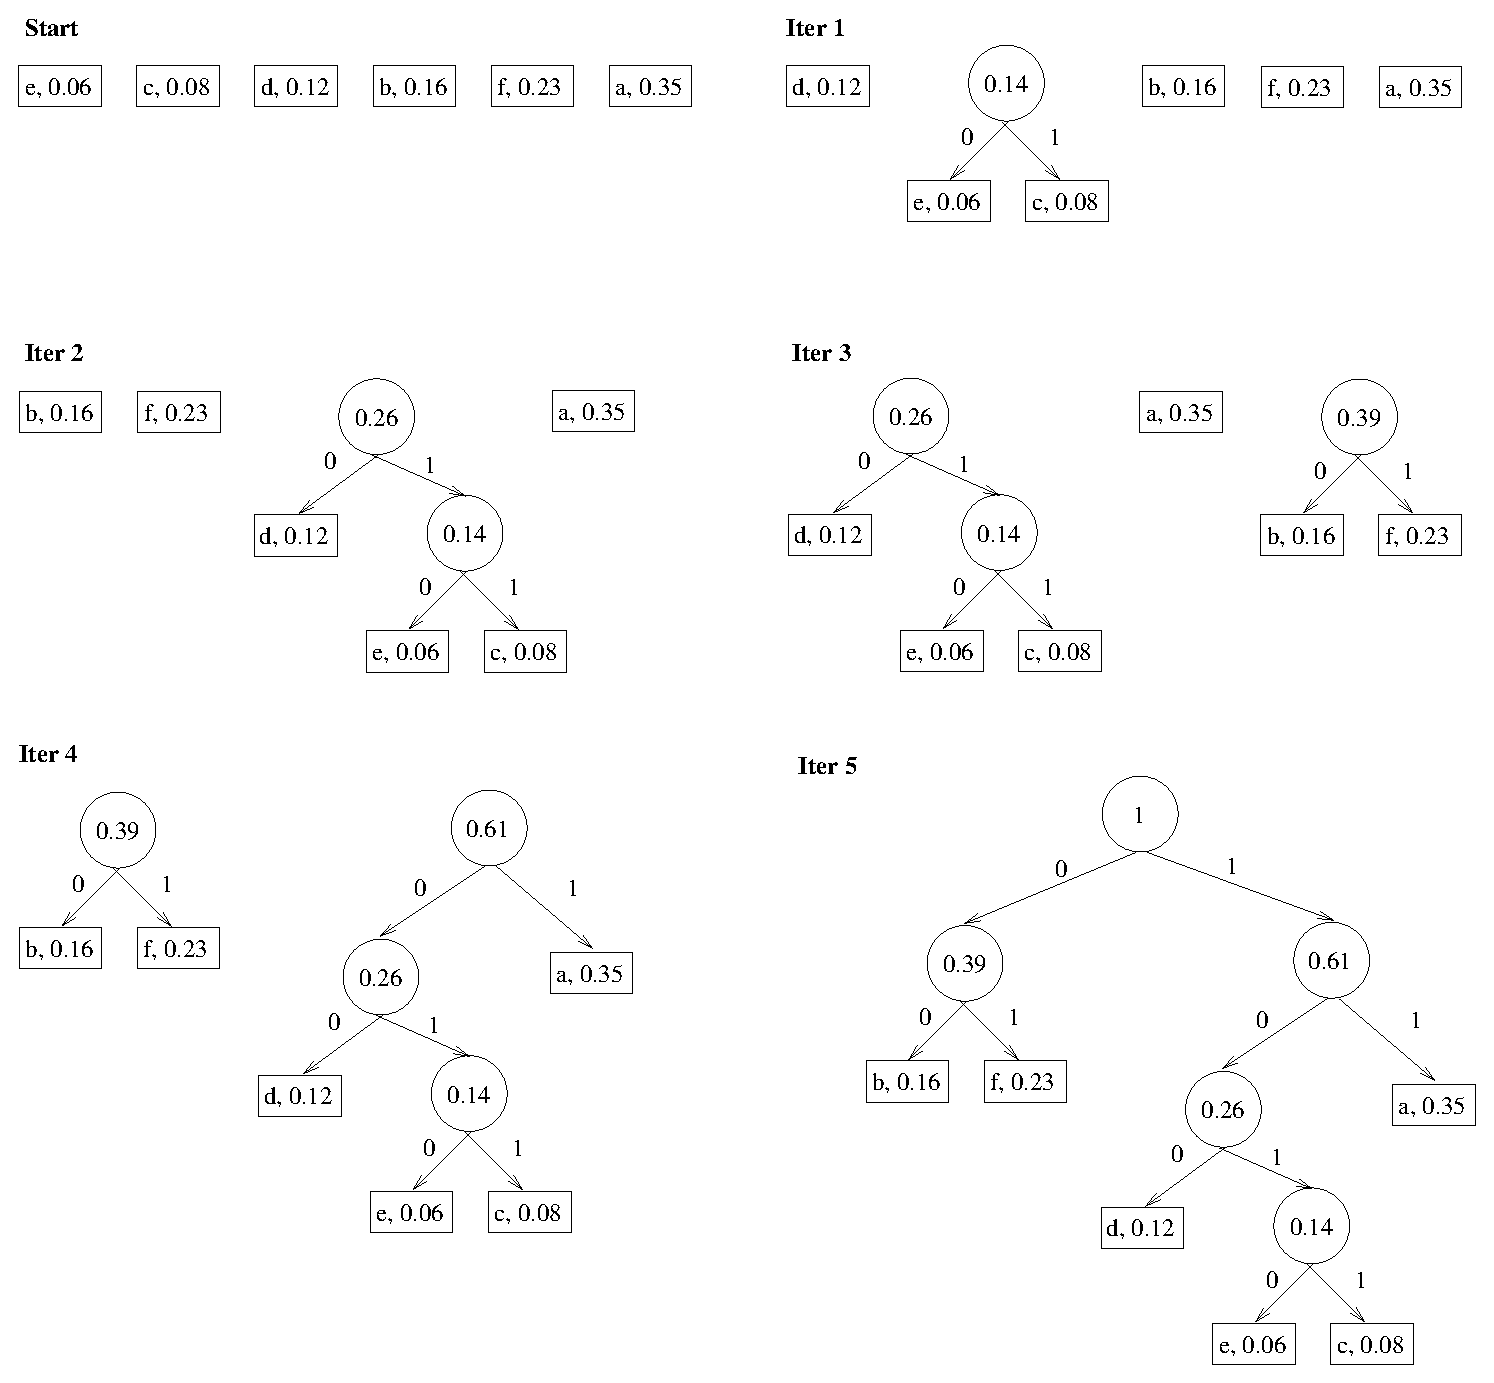
\includegraphics[scale=0.5]{huffman}
\caption{\label{fig:Huffman-Algorithm}Huffman Algorithm}
\end{figure}

\emph{This order is arbitrary; switching the left and rigth child of any node yields a different code of the same cost}

% Lemma would be better

\begin{proposition}
Given the probability is ...
\end{proposition}
\begin{proof}
{\color{red} TODO}
\end{proof}

The next theorem shows the optimality of the Huffman coding.

\begin{theorem}
If $C$ is a Huffman code then $C$ is compact.
\end{theorem}
\begin{proof}
{\color{red} TODO}
\end{proof}

{\color{red} TODO: Rewrite the following paragraphs}

\emph{So not only is this code optimal in the sense that no other feasible code performs better, but it is very close to the theoretical limit established by the entropy}

\emph{Although we have proved the theorem for a binary alphabet, the proof can be extended to establishing optimality of the Huffam coding algorithm for a D-ary alphabet as well.}

{\color{red} TODO: show how to extend the algorithm to D-ary codes}

\emph{Then -ary Huffman algorithm uses the {0, 1, ..., n-1} alphabet to encode message and build an n-ary tree [...] the same algorithm applies as for binary codes, except that the n least probable symbols are taken together , instead of just the 2 least probable. Note that for n greater than 2, not all sets of source words  can properly form an n-ary tree for Huffman coding. In this case, additional 0-probability place holders must be added. This is because the tree must form and n to 1 contractor; for binary coding, this is a 2 to 1 contractor, and any sized set can form such a contractor. If the number fo source words is congruent to 1 module n-1, then the set of source words will form a proper Huffman tree.}

{\color{red} Mention arithmetic coding}

%
% Section: Continuous Data
%

\section{Discretization Algorithms}
\label{sec:discretization_algorithms}

{\color{red} TODO: Rewrite this section.}

Let $\mathcal{X}$ a continuous random variable that follows a probability density function $P_\mathcal{X}$, and assume we have collected $n$ independent and identically distributed samples $\bold{x} = \{x_1, \ldots, x_n\}$ from $\mathcal{X}$. We are interested in computing the length of a compressed version of $\bold{x}$ using an optimal compressor. Unfortunately, and except for some degenerate distributions, there is no lossless compression algorithm that produces a string with fewer bits than encoding directly the elements $\bold{x}$. Compression algorithms for continuous data only work in case that the elements of $\bold{x}$ are not independent, as it is the case with images or sound. But, if this is not the case, the only option available to compress $\bold{x}$ is to use a lossy compression algorithm, where some information is lost.

We are looking for an algorithm to produce a finite non-overlapping partition of $m$ discrete intervals $D=\{ [d_o, d_1], (d_1, d_2], \ldots, (d_{m-1}, d_m] \}$, where $d_o = \min{\bold{x}_j}$, and $d_m = \max{\bold{x}_j}$, and $d_i < d_{i+1}$ for $i = 0, 1, \ldots, m-1$, assign a unique label to each interval, and encode the elements of $\bold{x}$ using this labeling schema. As compression algorithm we will use an optimal length code given the relative frequencies of the labels in the encoded vector. In this sense, our goal is to have a collection of intervals with sufficiently number of samples (so they are statistically significant) and that the distribution of frequencies resembles the original probability distribution $P_\mathcal{X}$.

A discretization algorithm is a mapping between a (possibly huge) number of numeric values and a reduced set of discrete values, and so, it is a process in which some information is potentially lost. The choice of discretization algorithm is something that could have a high impact in the practical computation of the nescience. We are interested in a discretization algorithm that produces a large number of intervals (low bias), with a large number of number of observations per interval (low variance). Common techniques include \emph{equal width discretization}, \emph{equal frequency discretization} and \emph{fixed frequency discretization}. However, these techniques require the optimization of an hyperparameter, and so, they are not suitable for our purposes.

In a \emph{proportional discretization approach} the number of intervals $m$ and the number of observations per interval $s$ are equally proportional to the number of observations $n$. The algorithm starts by sorting the values of $\bold{x}_j$ in ascending order and then discretizing them into $m$ intervals of approximately $s$ (possibly identical) values each. In this way, as the number of training observations increases, both interval frequency and number of intervals increases, taking advantage of the larger number of observations. In the same way, when the number of observations decreases, we reduce both.

\subsection{k-means Clustering}
\label{sec:kmeans_clustering}

K-means clustering is an algorithms that partitions n observations into k clusters in such a way that each observation belongs to the cluster with the nearest mean. In this way, we can replace the observation that belong to a cluster by its means, as a discretization. The optimization criteria in k-means is to minize the within-cluster variance. Given the fact that the problem is NP-Complete, some approximation algorithms are used instead.

{\color{red} TODO: Define the concept of Voronoi diagram / Voronoi cell}

\section*{References}

{\color{red} TODO: write this section}

In 1948, Claude E. Shannon published a paper entitled "A Mathematical Theory of Communication", where he established the foundations of a new discipline, later called \emph{information theory}.

Paper of Shannon ... Harley

Huffman -> D. A. Huffman. A method for the construction of minimum redundancy codes. Proc. IRE, 40:1098-1101, 1952.

The algorithm of huffman has been adapted from Cover. Here also you can find a proof that the algorithm is of order XX. 

Kraft's inequality was published by Leon G. Kraft in 1949 as part of his Master Thesis \cite{kraft1949device}. The inequality was independently rediscovered and proved for the general case of uniquely decodable codes by Brockway McMillan in 1956 \cite{mcmillan1956two}. The proofs contained in this book have been adapted from \cite{cover2012elements}.


The proof of proposition \ref{prop:maximum_entropy} has been adapted from \cite{abramson1963information}.
The proof of proposition 4.3.1 has been adapted from Abramson.

In the area of \emph{digital signal processing} \cite{gersho2012vector} it is common to apply a pre-processing step called \emph{quantization}, in which a large number of samples from a continuous signal are mapped into a finite number of representative values. It can be a \emph{scalar quantization} when the signal is one dimensional, or \emph{vector quantization} in case of a multidemensional signal. The optimization goal is to identify a (pre-defined) number of quantizied values such that the mean squared error between the selected values and the original signal is minimized. The problem is solved using the Lloyd-max algorithm \cite{lloyd1982least} (closely relted to the kmeans clustering algorithm \cite{} used in machine learning) in which the search space is paritioned in a collection of convex regions and their centroids used as quant, and then, are continously adapted until some stopping criteria is reached. Although it can be shown that the algorithm converges to the optimal solution that minimizes the mean squared error, the selected intervals cannot be used as estimation of the original probability distribution.




